% \documentclass[a4paper,10pt,draft]{thesis}
\usepackage{physics,amsmath, amsfonts, siunitx, amssymb, graphicx, slashed,subcaption}
\usepackage[utf8]{inputenc}
\usepackage[margin=1in]{geometry}
\usepackage[hidelinks]{hyperref}
\usepackage{xr-hyper}
\newcommand{\n}[1]{\nu_{#1}}
\newcommand{\na}{\nu_\alpha}
\newcommand{\nb}{\nu_\beta}
\newcommand{\ana}{\bar{\nu}_\alpha}
\newcommand{\an}[1]{\bar{\nu}_{\text{#1}}}
\newcommand{\anb}{\bar{\nu}_\beta}
\renewcommand{\a}{\alpha}
\renewcommand{\b}{\beta}
\newcommand{\ab}{\alpha\beta}


\renewcommand{\ne}{\nu_e}
\newcommand{\nm}{\nu_\mu}
\newcommand{\nt}{\nu_\tau}
\newcommand{\ns}{\nu_s}

\newcommand{\ane}{\bar{\nu}_e}
\newcommand{\anm}{\bar{\nu}_\mu}
\newcommand{\ant}{\bar{\nu}_\tau}
\newcommand{\ans}{\bar{\nu}_s}

\newcommand{\nee}{\nu_e \to \nu_e}
\newcommand{\nem}{\nu_e \to \nu_\mu}
\newcommand{\net}{\nu_e \to \nu_\tau}
\newcommand{\nes}{\nu_e \to \nu_s}

\newcommand{\nme}{\nu_\mu \to \nu_e}
\newcommand{\nmm}{\nu_\mu \to \nu_\mu}
\newcommand{\nmt}{\nu_\mu \to \nu_\tau}
\newcommand{\nms}{\nu_\mu \to \nu_s}



\newcommand{\Pee}{P_{e  e}}
\newcommand{\Pem}{P_{e  \mu}}
\newcommand{\Pet}{P_{e  \tau}}
\newcommand{\Pes}{P_{e  s}}

\newcommand{\Pme}{P_{\mu  e}}
\newcommand{\Pmm}{P_{\mu\mu}}
\newcommand{\Pmt}{P_{\mu  \tau}}
\newcommand{\Pms}{P_{\mu  s}}


\newcommand{\Pte}{P_{P_{\tau e}}}
\newcommand{\Ptm}{P_{\tau  \mu}}
\newcommand{\Ptt}{P_{\tau  \tau}}
\newcommand{\Pts}{P_{\mu  s}}

\newcommand{\Paeae}{P_{\bar{e}  \bar{e}}}
\newcommand{\Paeam}{P_{\bar{e}  \bar{\mu}}}
\newcommand{\Paeat}{P_{\bar{e}  \bar{\tau}}}
\newcommand{\Paeas}{P_{\bar{e}  \bar{s}}}

\newcommand{\Pamae}{P_{\bar{\mu}  \bar{e}}}
\newcommand{\Pamam}{P_{\bar{\mu}  \bar{\mu}}}
\newcommand{\Pamat}{P_{\bar{\mu}  \bar{\tau}}}
\newcommand{\Pamas}{P_{\bar{\mu}  \bar{s}}}


\newcommand{\Patae}{P_{\bar{\tau}  \bar{e}}}
\newcommand{\Patam}{P_{\bar{\tau}  \bar{\mu}}}
\newcommand{\Patat}{P_{\bar{\tau}  \bar{\tau}}}
\newcommand{\Patas}{P_{\bar{\mu}  \bar{s}}}

\renewcommand{\th}[1][]{%
  \theta\ifx\\#1\\\else_\text{#1}\fi
}
\newcommand{\thm}[1][]{%
  \theta^\text{M}\ifx\\#1\\\else_\text{#1}\fi
}
\renewcommand{\t}[1]{\text{{#1}}}
\newcommand{\avg}[1]{\left\langle {#1} \right \rangle}
\newcommand*{\dm}[1][]{%
  \Delta m^2\ifx\\#1\\\else_\text{#1}\fi
}
\newcommand{\zreco}{\cos{(\theta_z^{reco})}}
\newcommand{\ztrue}{\cos{(\theta_z^{true})}}
\newcommand{\z}{\cos{(\theta_z)}}
\newcommand{\Ereco}{E^{reco}}
\newcommand{\Etrue}{E^{true}}
\newcommand{\Aeff}{A^\text{eff}}
\newcommand{\emm}{\epsilon_{\mu\mu}}
\newcommand{\emt}{\epsilon_{\mu\tau}}
\newcommand{\eet}{\epsilon_{e\tau}}
\newcommand{\eem}{\epsilon_{e\mu}}
\newcommand{\ett}{\epsilon_{\tau\tau}}
\newcommand{\ep}{\epsilon^\prime}

% \begin{document}

\section{Neutrino Mixing}\label{ch:oscillation}

%\subsection{Mass Generation}
In the Standard Model, fermion masses are generated by the Higgs mechanism through Yukawa couplings with the fermions right and left-handed components.
All neutrinos are left-handed and all antineutrinos are right-handed. Thus, neutrinos are massless since they do not undergo the Higgs mechanism.
Additionally, all terms of a Lagrangian that we construct must respect the gauge invariance. This removes the possibility of the neutrino mass to be 
generated at loop level because any such attempt will violate the total lepton number by two units.
In order to keep our theory renormalizable, we have one option left: introducing additional fermions. 

We consider a right-handed neutrino field, $\nu_R$. Since the electroweak gauge group $\text{SU}(2)_L \times U(1)_Y$ only couple to 
left-handed particles and right-handed antiparticles, $\nu_R$ transforms as a singlet under the SM symmetry 
group $\mathrm{SU}(3)_{\mathrm{C}} \times \mathrm{SU}(2)_{L} \times \mathrm{U}(1)_{Y}$. 
This neutrino field is \emph{sterile} since it doesn't participate any of the SM interactions. 

We extend the Standard Model by adding a right-handed component of this field with neutrino Yukawa couplings $Y_{\alpha \beta}^{\prime \nu}$ to the Higgs-lepton Yukawa Lagrangian from Eq.~\ref{eq:YukawaLagrangian} 
\begin{align}
    \mathcal{L}_{H}=-\left( \frac{v + H}{\sqrt{2}} \right) \left[\ell_{\alpha L}^{\prime} Y_{\alpha \beta}^{\prime \ell} \ell_{\beta R}^{\prime} + \nu_{\alpha L}^{\prime} Y_{\alpha \beta}^{\prime \nu} \nu_{\beta R}^{\prime}\right]
\end{align}
Similar to how we diagonalized the lepton Yukawa couplings $Y_{\alpha \beta}^{\prime \ell}$ in Eq.~\ref{eq:leptonYukawaDiag}, we diagonalize $Y_{\alpha \beta}^{\prime \nu}$ as
\begin{align}
    V_{\alpha k L}^{\nu \dagger} Y^{\prime \nu}_{\alpha \beta} V_{\beta j R}^{\nu}=Y^{\nu}_{kj} \,.
\end{align}
Now we introduce a crucial difference between the properties of the charged lepton and the neutrino fields.
While the charged lepton flavor eigenstate was uniquely determined by its mass eigenstate, the neutrino flavor is a superposition of mass eigenstates. This is because neutrinos are indirectly detected via the observation of its associated charged lepton, so there is no requirement of neutrino flavor eigenstates to have a definite mass. The flavor of a neutrino is then, by definition, the flavor of the associated charged lepton. This is commonly introduced as giving the mass eigenstates Latin numerals and letters, while the flavor eigenstates stay as Greek letters.

So, let the neutrino field with chriality $X$ be denoted $\nu_X$, with components having Latin numerals to distinguish them from the flavour components, i.e 
\begin{align}\label{eq:nu_rotation}
    \nu_{k X} =  V_{k\beta X}^{\nu \dagger} \nu_{\beta X}^\prime\,.
\end{align}
The diagonalized Lagrangian now takes the form 
\begin{align}
    \mathcal{L}_{H} &= -\left( \frac{v + H}{\sqrt{2}} \right) \left[\ell_{\alpha L}^{\prime} Y_{\alpha \beta}^{\prime \ell} \ell_{\beta R}^{\prime} + \nu_{\alpha L}^{\prime} Y_{\alpha \beta}^{\prime \nu} \nu_{\beta R}^{\prime}\right] \nonumber \\
    &= -\left( \frac{v + H}{\sqrt{2}} \right) \left[\ell_{\alpha L}^{\prime} V_{\alpha \beta L}^{\ell} Y_{\alpha \beta}^{ \ell} V_{\alpha \beta R}^{\ell \dagger} \ell_{\beta R}^{\prime}\right. \nonumber \\
    &\hspace{5.7em}+\left. \nu_{\alpha L}^{\prime} V_{\alpha k L}^{\nu} Y_{kj}^{\nu} V_{\beta j  R}^{\nu \dagger} \nu_{\beta R}^{\prime}\right] \nonumber \\
    &= -\left( \frac{v + H}{\sqrt{2}} \right) \left[\ell_{\alpha L}^\dagger Y_{\alpha \beta}^{ \ell} \ell_{\beta R} + \nu_{k L}^{\dagger} Y_{kj}^{ \nu} \nu_{j R}\right] \nonumber \\
    &= -\left( \frac{v + H}{\sqrt{2}} \right) \left[\bar{\ell}_{\alpha L} Y_{\alpha \beta}^{ \ell} \ell_{\beta R} + \bar{\nu}_{k L} Y_{kj}^\nu \nu_{j R}\right]
\end{align}
By construction, $Y^\ell_{\alpha \beta}$ and $Y^\nu_{kj}$ are diagonal, so we write them as $y_{\alpha}^{\ell} \delta_{\alpha \beta}$ and $y_{k}^{\nu} \delta_{k j}$ respectively, leaving the Lagrangian as 
\begin{align}\label{eq:L_H}
    \mathcal{L}_{H} 
    &=-\left( \frac{v + H}{\sqrt{2}} \right) \left[\bar{\ell}_{\alpha L} y_{\alpha}^{\ell} \delta_{\alpha \beta} \ell_{\beta R} + \bar{\nu}_{k L} y_{k}^{\nu} \delta_{k j} \nu_{j R}\right] \nonumber \\
    &=-\left( \frac{v + H}{\sqrt{2}} \right) \left[\bar{\ell}_{\alpha L} y_{\alpha}^{\ell}  \ell_{\alpha R} + \bar{\nu}_{k L} y_{k}^{\nu} \nu_{k R}\right] \nonumber \\
    &=-\left( \frac{v + H}{\sqrt{2}} \right) \left[ y_{\alpha}^{\ell}  \bar{\ell}_{\alpha L}\ell_{\alpha R} +  y_{k}^{\nu}\bar{\nu}_{k L} \nu_{k R}\right] 
\end{align}

Now, the Dirac neutrino field is
\begin{align}
    \nu_k = \nu_{kL} + \nu_{kR}\,.
\end{align}
Multiplying $\nu_k$ with its conjugate $\bar{\nu}_k$, we get 
\begin{align}
    \bar{\nu}_k \nu_k 
    & = \bar{\nu}_{k L} \nu_{k L} +\bar{\nu}_{k R}\nu_{k L} + \bar{\nu}_{k L}\nu_{k R} + \bar{\nu}_{k R}\nu_{k R} \nonumber \\
    & = \bar{\nu}_{k L}\nu_{k R} + \bar{\nu}_{k R}\nu_{k L} \nonumber \\
    & = \bar{\nu}_{k L}\nu_{k R} + \t{h.c.}
\end{align}
The same calculation for the charged lepton field yields the same result for $\ell_k$. Substituting this result and expanding the Higgs vacuum expectation value $v$ into the fields gives us
\begin{align}
    \mathcal{L}_{H} 
    &=-\left( \frac{v + H}{\sqrt{2}} \right) \left[ y_{\alpha}^{\ell}   \bar{\ell}_\alpha \ell_\alpha  +  y_{k}^{\nu} \bar{\nu}_k \nu_k \right] \nonumber \\
    &=- \frac{y_{\alpha}^{\ell} v}{\sqrt{2}}   \bar{\ell}_\alpha \ell_\alpha   -  \frac{ y_{k}^{\nu} v}{\sqrt{2}} \bar{\nu}_k \nu_k  - \frac{y_{\alpha}^{\ell}}{\sqrt{2}}   \bar{\ell}_\alpha \ell_\alpha H  -  \frac{ y_{k}^{\nu}}{\sqrt{2}} \bar{\nu}_k \nu_k H\,.
\end{align}
Thus, this extension to the SM generates neutrino masses at electroweak symmetry breaking by the Higgs mechanism with mass terms
\begin{align}
    m_k = \frac{y_k^\nu v}{\sqrt{2}}\,.
\end{align}

\subsection{The mixing matrix}
Substituting the new transformation from Eq.~\ref{eq:nu_rotation} into the weak charged current, we get
\begin{align}\label{eq:j_CC2}
    j^\rho_L &= 2\bar{\nu}^\prime_{\alpha L} \gamma^\rho \ell_{\alpha L}^\prime \nonumber \\
             &= 2\bar{\nu}_{k L} V^{\prime \nu \dagger}_{k \alpha}V^{\prime \ell}_{\alpha \alpha} \gamma^\rho  \ell_{\alpha L}
\end{align}

Now, the current in Eq.~\ref{eq:j_CC2} conserves lepton number, since the neutrino field with flavor $\alpha$ only couples to the lepton field with flavor $\alpha$. 
Thus, neutrino interactions still conserve lepton number.
However, the Higgs-lepton Yukawa Lagrangian 
in Eq.~\ref{eq:L_H} violates lepton number conservation since it couples the charged lepton flavor $\alpha$ to the neutrino mass eigenstate $k$, which is a superposition of flavors. 
There is no transformation that leaves both the interaction and kinetic Lagrangian invariant, thus violating this symmetry.


Call $V^{\prime \nu \dagger}_{k \alpha}V^{\prime \ell}_{\alpha \alpha} = U^\dagger_{k \alpha}$. We will refer to the matrix $U$ built by the components $U_{k \alpha}$ as the
Pontecorvo-Maki-Nakagawa-Sakata (PMNS) matrix. %TODO: source
We now have 
\begin{align}\label{eq:j_CC3} %TODO: put sums on all above?
    j^\rho_L &= 2 \sum_\alpha \sum_k U^\dagger_{\alpha k} \bar{\nu}_{k L} \gamma^\rho  \ell_{\alpha L}\,.
\end{align}

What form does this new matrix $U$ take? By construction, it provides the unitary transformation between the flavor and mass bases.
Any unitary $3\times3$ matrix can be parametrized using three mixing angles and six phases. However, not all phases affect the 
charged and weak currents and are thus not observable. Moreover, both the Lagrangian and the currents are invariant under global $U(1)$ transformations,
leaving only one physical phase for us to measure. Thus we are down to four degrees of freedom in the three dimensional case: three mixing angles
of the form $\sin{(\theta_{ij})}/\cos{(\theta_{ij})} = s_{ij}/c_{ij}$, and one phase of the form $e^{i\delta}$.

We construct the PMNS matrix using the rotation matrixes from $SO(3)$ as
\begin{align}
    U &= R_{23}R_{13,\delta_{\text{CP}}}R_{12} \nonumber \\
      & = 
    \begin{pmatrix}1 & 0 & 0 \\ 0 & c_{23} & s_{23} \\ 0 & -s_{23} & c_{23}\end{pmatrix}
\begin{pmatrix}c_{13} & 0 & s_{13} e^{-i \delta_{\mathrm{CP}}} \\ 0 & 1 & 0 \\ -s_{13} e^{i \delta_{\mathrm{CP}}} & 0 & c_{13}\end{pmatrix}
\begin{pmatrix}c_{12} & s_{12} & 0 \\ -s_{12} & c_{12} & 0 \\ 0 & 0 & 1\end{pmatrix}\,.
\end{align}
The term $\delta_\text{CP}$ determines the degree of charge-parity violation. In this work, we will assume CP invariance by always
setting $\delta_{CP} = \SI{0}{\degree}$. Thus,

\begin{align}
    U &=
    \begin{pmatrix}1 & 0 & 0 \\ 0 & c_{23} & s_{23} \\ 0 & -s_{23} & c_{23}\end{pmatrix}
\begin{pmatrix}c_{13} & 0 & s_{13} \\ 0 & 1 & 0 \\ -s_{13}  & 0 & c_{13}\end{pmatrix}
\begin{pmatrix}c_{12} & s_{12} & 0 \\ -s_{12} & c_{12} & 0 \\ 0 & 0 & 1\end{pmatrix} \nonumber \\
    &= 
    \begin{pmatrix}c_{12} c_{13} & s_{12} c_{13} & s_{13} \\ 
        -s_{12} c_{23}-c_{12} s_{23} s_{13} & c_{12} c_{23}-s_{12} s_{23} s_{13} & s_{23} c_{13} \\ 
        s_{12} s_{23}-c_{12} c_{23} s_{13}  & -c_{12} s_{23}-s_{12} c_{23} s_{13} & c_{23} c_{13}
    \end{pmatrix}\,.
\end{align}

In this work, we will be using the best-fit values from~\cite{nufit} with the exception of the CP-violating phase $\delta_\text{CP}$. The $90\% $ CL values are
\begin{align}\label{eq:nufitparams}
    \theta_{12} = \SI{33.44}{\degree},\hspace{1em} \theta_{13} = \SI{8.57}{\degree},\hspace{1em} \theta_{23} = \SI{49.2}{\degree}, \hspace{1em} \delta_\text{CP} = 0\,.
\end{align}
The PMNS matrix is then real, with numerical values 
\begin{align}\label{eq:Uvalues}
    U = \begin{pmatrix}
        U_{e 1} & U_{e2} & U_{e3} \\
        U_{\mu 1} & U_{\mu 2} & U_{\mu 3} \\
        U_{\tau 1} & U_{\tau 2} & U_{\tau 3}
    \end{pmatrix} 
    = \begin{pmatrix}
        0.825 & 0.545 & 0.149 \\
        -0.455 & 0.485 & 0.746 \\
        0.334 & -0.684 & 0.649
    \end{pmatrix} \,.
\end{align}
In our study, we will only use neutrinos originating from conventional cosmic ray interactions in the atmosphere. 
In this so-called atmospheric neutrinos, $\nm$ are the most abundant, while the $\nt$ flux is neglible. We see that $U_{\mu\tau}$ is the largest $U_{\mu\beta}$ term,
suggesting that $\nm$ primarily mixes into $\nt$, at least in vacuum. It turns out that matter effects indeed preserves this ordering, making the $\nm \to \nt$ transition
the most abundant. This means we will be able to stringently constrain parameters relating to $\mu\tau$ mixing.

\subsection{Neutrino Propagation}
Since we now know how the neutrino mass and flavor eigenstates combine, and have an expression for the flavor interaction with 
the neutrino's charged lepton partner, we are now ready to study the flavor oscillations themselves.

Now, the Fourier expansion of the field operator $\bar{\nu}_{k L}$ in the current of Eq.~\ref{eq:j_CC3} contains creation operators $a^\dagger_{\nu_k}$
of massive neutrinos with mass $m_k$. This means that the summation over the mass index $k$ constructs a flavor neutrino, which interacts with the charged lepton field $\ell_{\a L}$.
In other words, the charged current generates a flavor neutrino $\na$, which is a superposition of the mass eigenstates 
$\nu_k$ with weights $U_{\a k}^\dagger$. In the ket-formalism, we express this as
\begin{align}\label{eq:osc_1}
    \ket{\na} = \sum_k U^\dagger_{\a k} \ket{\nu_k}\,.
\end{align}
It is the mass eigenstates $\ket{\nu_k}$ that are eigenstates of the Hamiltonian, with eigenvalues
\begin{align}\label{eq:disp}
    E_k = \sqrt{\vec{p}^2 + m_k^2}\,.
\end{align}
The solution to the time-dependent Schrödinger equation 
\begin{align}\label{eq:TDSE}
    i \dv{}{t} \ket{\nu_k(t)} = H_0\ket{\nu_k(t)}\,,
\end{align}
where $H_0$ is the Hamiltonian and the subscript signifies that we are in vacuum. 

The solution to Eq.~\ref{eq:TDSE} gives ut the time evolution
in the form of plane wave solutions: 
\begin{align}
    \ket{\nu_k(t)} = e^{-iE_kt}\ket{\nu_k}\,.
\end{align}
Inserting the plane wave solution into Eq.~\ref{eq:osc_1}, we get 
\begin{align}\label{eq:nat}
    \ket{\na(t)} = \sum_k U^\dagger_{\a k} e^{-iE_kt}\ket{\nu_k}\,.
\end{align}
Now we know how to evolve and combine the mass eigenstates to form a flavor eigenstate, but how about the reverse?
 We swap the index $k\to j$ in Eq.~\ref{eq:osc_1} and multiply by $U_{\a k}$:
\begin{align}\label{eq:osc_k}
    \sum_\a U_{\a k}\ket{\na} &= \sum_{\alpha, j} U_{\a k} U_{\a j}^\dagger \ket{\nu_j} \nonumber \\
    \sum_\a U_{\a k}\ket{\na} &= \sum_{j} \delta_{kj} \ket{\nu_j} \nonumber \\
    \sum_\a U_{\a k}\ket{\na} &= \ket{\nu_k}\,,
\end{align}
where we have used the unitarity of the leptonic mixing matrix. Eqs.~\ref{eq:osc_1} and \ref{eq:nat} yield 
\begin{align}
    \ket{\na(t)} &= \sum_k U^\dagger_{\a k} e^{-iE_kt}\ket{\nu_k} \nonumber \\
    \ket{\na(t)} &= \sum_k U^\dagger_{\a k} e^{-iE_kt}\left(\sum_\b U_{\b k}\ket{\nb}\right) \nonumber \\
    \ket{\na(t)} &= \sum_{k,\b} U^\dagger_{\a k}U_{\b k} e^{-iE_kt} \ket{\nb}\,.
\end{align}
The probability of the flavor transition $\na \to \nb$ at time $t$ is $\abs{\bra{\nb}\ket{\na (t)}}^2$:
\begin{align}
    P_{\na \to \nb}(t) = \sum_{k,j} U^\dagger_{\a k}U_{\b k}U^*_{\b j}U_{\a j} e^{-i(E_k-E_j)t}\,.
\end{align}

We assume the neutrino masses $m_k$ to be extremely small compared to their associated energies $E_k$. 
Thus, $v\sim 1$, and $\abs{\vec{p}} \sim E$ making the energy-dispersion relation of Eq.~\ref{eq:disp} to first order:
\begin{align}\label{eq:ultra_rel}
    E_k &= \sqrt{\vec{p}^2 + m_k^2} \nonumber \\
        &= \vec{p}^2\sqrt{1 + \frac{m_k^2}{\vec{p}^2}} \nonumber \\
        &\approx E + \frac{m_k^2}{2E}
\end{align}
Hence, the exponential can be simplified, and simplifying the notation $P_{\na \to \nb}(t) \to P_{\ab}(t)$ we get 
\begin{align}
    P_{\ab}(t) = \sum_{k,j} U^\dagger_{\a k}U_{\b k}U^\dagger_{\b j}U_{\a j} e^{-i(m_k^2-m_j^2)t/2E}\,.
\end{align}
Now, our approximation $v\approx 1$ implies $x\approx t $, thus
\begin{align}
    P_{\ab}(x) &= \sum_{k,j} U^\dagger_{\a k}U_{\b k}U^\dagger_{\b j}U_{\a j} e^{-i(m_k^2-m_j^2)x/2E} \nonumber \\
                       &= \sum_{k,j} U^\dagger_{\a k}U_{\b k}U^\dagger_{\b j}U_{\a j} \exp(-i\frac{\dm_{kj}x}{2E})\,,
\end{align}
where we in the last step have defined the \emph{mass squared-difference} $\dm_{kj} = m_k^2 - m_j^2$. Since the oscillation probability depends on this quantity
rather than the individual masses, it is impossible
to measure the mass $m_k$ through neutrino oscillations.
Squaring the unitarity condition $\sum_k U_{\a k}U_{\b k}^\dagger = \delta_{\a \b}$ yields 
\begin{align}
    \sum_k \abs{U_{\a k}}^2\abs{U_{\b k}}^2 = \delta_{\a \b} - 2 \sum_{k>j}\Re[U_{\a k}^\dagger U_{\b k} U_{\a j} U_{\b j}^\dagger]
\end{align}
Since we take the PMNS matrix to be real and thus Hermitian, we drop the complex transpose in the following calculation. We have
\begin{align}\label{eq:Pab}%TODO: shorten?
    P_{\ab} &= \sum_{k,j} U_{\a k}U_{\b k}U_{\b j}U_{\a j} \exp(-i\frac{\dm_{kj}x}{2E}) \nonumber \\
            &=  \sum_k \abs{U_{\a k}}^2\abs{U_{\b k}}^2 + \nonumber \\
            &\hspace{2em}+ \sum_{k \neq j} U_{\a k}U_{\b k}U_{\b j}U_{\a j} \exp(-i\frac{\dm_{kj}x}{2E}) \nonumber \\
            &= \delta_{\a \b} - 2 \sum_{k>j}U_{\a k} U_{\b k} U_{\b j} U_{\a j} \nonumber \\
            & \hspace{3em}+\sum_{k \neq j} U_{\a k}U_{\b k}U_{\b j}U_{\a j} \exp(-i\frac{\dm_{kj}x}{2E}) \nonumber \\
            &= \delta_{\a \b} - 2 \sum_{k>j}U_{\a k} U_{\b k} U_{\b j} U_{\a j} \nonumber \\
            &\hspace{3em}+ 2\sum_{k > j} U_{\a k}U_{\b k}U_{\b j}U_{\a j} \exp(-i\frac{\dm_{kj}x}{2E}) \nonumber \\
            &= \delta_{\a \b} - 2\sum_{k > j} U_{\a k}U_{\b k}U_{\b j}U_{\a j} \left[1-\exp(-i\frac{\dm_{kj}x}{2E})\right] \nonumber \\
            &= \delta_{\a \b} - 2\sum_{k > j} U_{\a k}U_{\b k}U_{\b j}U_{\a j} \left[1-\cos(\frac{\dm_{kj}x}{2E})\right] \nonumber \\
            &= \delta_{\a \b} - 2\sum_{k > j} U_{\a k}U_{\b k}U_{\b j}U_{\a j} \sin^2{\left(\frac{\dm_{kj}x}{4E}\right)}\,,
\end{align}
which is the probability of neutrino vacuum oscillations. %TODO: maybe plot?
The calculation for antineutrinos yield the same result if one continues to assume the Hermicity of the mixing matrix. 
In Fig.~\ref{fig:vac_osc}, we show the energy spectra of these oscillations in the low \si{\GeV} range for neutrinos that travel \SI{12000}{\km}\footnote{This baseline
is approximately the Earth diameter, and will be the maximum travel distance which we will use later on.}.
In the left-most panel, we see a supressed $\nu_\mu \to e$ transition. We can understand this behavior by studying Eq.~\ref{eq:Pab} and the 
numerical values of the mixing matrix in Eq.~\ref{Uvalues}.
\si{\GeV} oscillations are driven by the $\dm[31]$ mass-squared difference. Hence, the most important mixing matrix 
elements for $P_{\a\b}$ are $U_{\a3}, U_{\a1}$ and $U_{\b3}, U_{\b1}$. The smallness of $U_{e3}$ then supresses the
amplitude of $\Pme$.
\begin{figure}
    \centering
    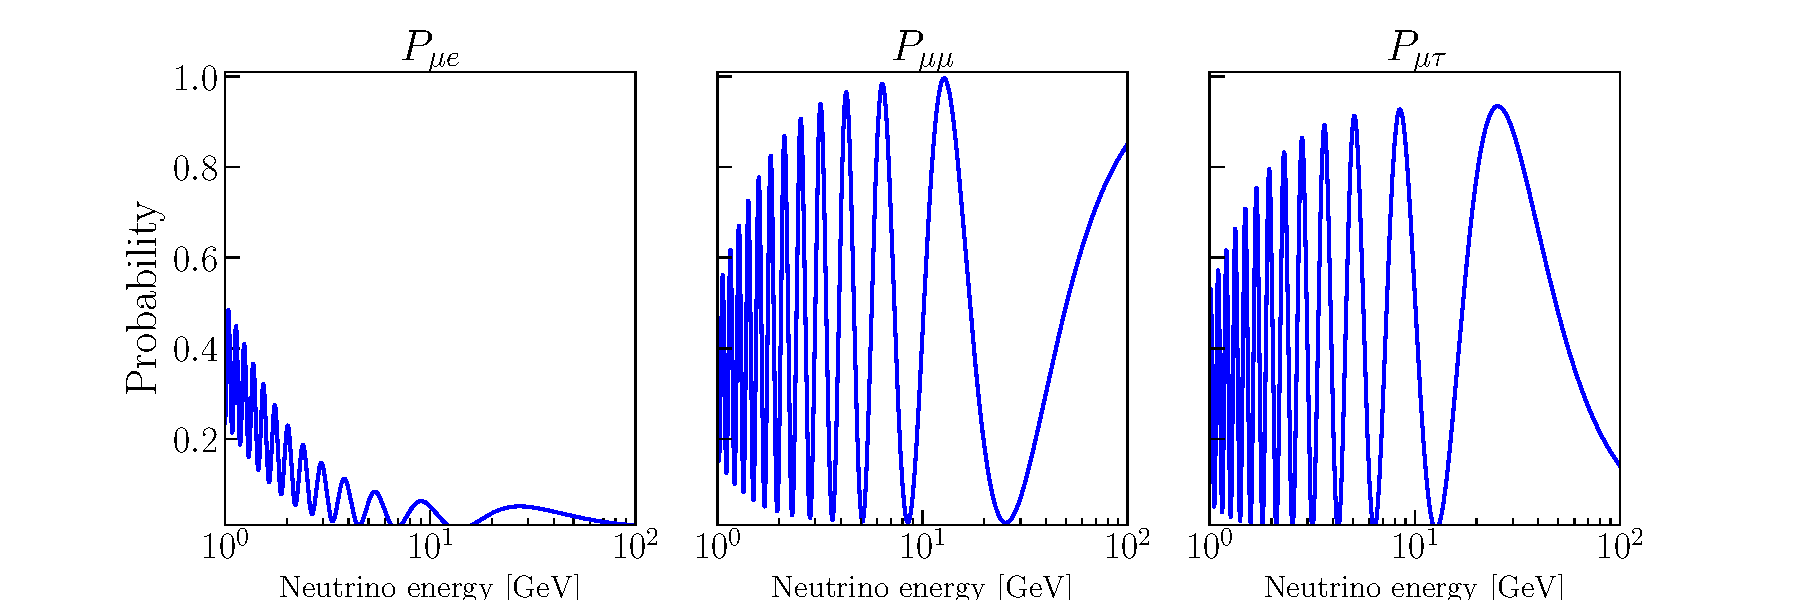
\includegraphics[width=0.9\textwidth]{figures/vac_osc.pdf}
    \caption{$\nm$ vacuum oscillations from Eq.~\ref{eq:Pab}}\label{fig:vac_osc}
\end{figure}

For our purposes, the probabilities in Eq.~\ref{eq:Pab} are rather uninteresting, since they are only valid in vacuum.
Despite this fact, this form elucidates an important aspect of neutrino oscillations. The mixing matrix elements
determine the amplitude of the oscillations, while the mass-squared differences together with the ratio $L/E$ determine the 
frequency. 

\subsection{Effective Potentials}

\begin{figure}
    \centering
    \begin{subfigure}{0.3\textwidth}
        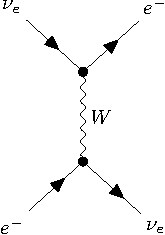
\includegraphics[width=0.9\textwidth]{figures/w-boson.pdf} 
        \caption{Charged current weak interaction between an electron neutrino and an electron,
        mediated by either a $W^+$ or $W^-$ boson.}
    \end{subfigure}
    \quad
    \begin{subfigure}{0.3\textwidth}
        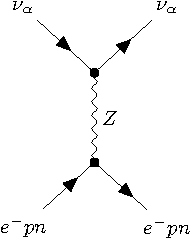
\includegraphics[width=1\textwidth]{figures/z-boson.pdf} 
        \caption{Neutral current weak interaction between a neutrino of any flavor and a Earth-like fermion,
        mediated by a neutral $Z$ boson.}
    \end{subfigure}%TODO: they are different sizes
    \caption{Feyman diagrams showing the two interactions that neutrinos participate in according to the Standard Model.}\label{fig:w_and_z}
\end{figure}
In this work, we are concerned about the interactions with the neutrino and Earth-like matter, i.e.~electrons, protons, and neutrons. 
The possible interactions are shown in Fig.~\ref{fig:w_and_z}. The left panel shows that the only flavor that can go through charged current (CC) 
interactions is the electron flavor. This is because the Earth doesn't consist of any muons or tau particles. 
The right panel shows any neutrino flavor interaction via the neutral current (NC) with Earth-like matter\footnote{The Earth is entirely composed
of electrons, protons, and neutrons. Thus, the fundamental particles composing Earth are electrons, and up and down quarks. We refer to this as \emph{Earth-like matter}.}, mediated by the neutral $Z$ boson
The interaction mediated by the $W$ boson will give rise to a effective matter potential $V_{CC}$, while
the $Z$ boson is responsible for $V_{NC}$. Our task is now to find expressions for these.

We start with the effective Hamiltonian for the CC process. The Feynman rules for the left panel give us 
\begin{align}
    H_{CC} = \frac{G_F}{\sqrt{2}}\left[ \bar\ne \gamma^\rho\, (1- \gamma^5)\, e \right] \left[\bar e \,\gamma_\rho\, (1- \gamma^5)\, \ne \right]
\end{align}
By using the Fierz transformation 
\begin{align}
    \mathcal{L}^{V-A}(\psi_1,\psi_2,\psi_3,\psi_4) = \mathcal{L}^{V-A}(\psi_1,\psi_4,\psi_3,\psi_2)\,,
\end{align}
we can permute the terms inside the brackets, yielding
\begin{align}\label{eq:H_fierz}
    H_{CC} = \frac{G_F}{\sqrt{2}}\left[ \bar\ne \gamma^\rho\, (1- \gamma^5)\, \ne \right] \left[\bar e \,\gamma_\rho\, (1- \gamma^5)\, e \right]\,.
\end{align}
Now, lets consider a finite volume $V$ with electron states defined as 
\begin{align}\label{eq:e_states}
    \ket{e(p_e,h_e)} = \frac{1}{2E_eV}a_e^{(h_e)\dagger}(p_e)\ket{0}\,,
\end{align}
i.e. using the creation operator $a_e^{(h_e)\dagger}(p_e)$ to create electron states from vacuum with momenta $p_e$, energy $E_e$, and helicity $h_e$.
The density distribution of electrons in $V$ is $f(E_e,T)$, which we normalize to the total number of electrons as we integrate out the momenta $p_e$:
\begin{align}\label{eq:e_density}
    \int \dd p_e^3 f(E_e,T) = N_e V = n_e
\end{align}
Here, the electron density $N_e$ will ultimately determine the strength of the effective matter potential. 
To obtain the average effective Hamiltonian, project it on the electron states in Eq.~\ref{eq:e_states} and integrate over the density and sum over the helicities:

\begin{align}\label{eq:avg_H1}
    \avg{H_{CC}} &= \int \dd p_e^3 \bra{e(p_e,h_e)} \times \frac{1}{2} \sum_{h_e} H   f(E_e,T) \ket{e(p_e,h_e)} \nonumber \\
           &= \frac{G_F}{\sqrt{2}} \int \dd p_e^3 \bra{e(p_e,h_e)} \left[ \bar\ne \gamma^\rho\, (1- \gamma^5)\, \ne \right]  f(E_e,T) \times \frac{1}{2} \sum_{h_e} \left[\bar e(x) \,\gamma_\rho\, (1- \gamma^5)\, e(x) \right] \ket{e(p_e,h_e)} \nonumber \\
           &= \frac{G_F}{\sqrt{2}} \bar\ne \gamma^\rho\, (1- \gamma^5)\, \ne \int \dd p_e^3  f(E_e,T) \times \frac{1}{2} \sum_{h_e} \bra{e(p_e,h_e)} \bar e(x) \,\gamma_\rho\, (1- \gamma^5)\, e(x)   \ket{e(p_e,h_e)}\,.
\end{align}
First, calculate the sum using trace technology %TODO: explain this more
\begin{align}\label{eq:helicity_sum}
    \frac{1}{2} \sum_{h_e} \bra{e(p_e,h_e)} \bar e(x) \,\gamma_\rho\, (1- \gamma^5)\, e(x)   \ket{e(p_e,h_e)} &= \frac{1}{4E_e V} \sum_{h_e} \bar{u}_e^{h_e}(p_e) \,\gamma_\rho\, (1- \gamma^5)\, u_e^{h_e}(p_e) \nonumber \\
    &= \frac{1}{4 E_e V} \Trace{\left[ \sum_{h_e} \bar{u}_e^{h_e}(p_e) u_e^{h_e}(p_e) \,\gamma_\rho\, (1- \gamma^5)\, \right]} \nonumber \\
    &= \frac{1}{4 E_e V} \Trace{\left[ (\slashed{p}_e + m_e ) \,\gamma_\rho\, (1- \gamma^5)\, \right]} \nonumber \\
    &= \frac{(p_e)_\rho}{E_e V}\,.
\end{align}
Eq.~\ref{eq:avg_H1} now becomes 
\begin{align}\label{eq:avg_H2}
    \avg{H_{CC}} &= \frac{G_F}{\sqrt{2}E_e V} \bar\ne \, (1- \gamma^5)\, \ne \int \dd p_e^3\, \slashed{p}_e\, f(E_e,T)\,.
\end{align}
Expand the integral, and use the fact that $\vec{p}_e$ is odd:
\begin{align}
    \int \dd p_e^3\, \slashed{p}_e\, f(E_e,T) &= \int \dd p_e^3\, f(E_e,T) (\gamma^0 E_e - \vec{p}_e \cdot \vec{\gamma}) \nonumber \\
                                              &= \int \dd p_e^3\, f(E_e,T) \gamma^0 E_e \nonumber \\
                                              &= \gamma_0 E_e N_e V\,.
\end{align}
Inserting this into Eq.~\ref{eq:avg_H2}, we have
\begin{align}
    \avg{H_{CC}} &= \frac{G_F N_e}{\sqrt{2}} \bar{\nu}_e \, (1- \gamma^5)\, \ne \gamma_0 \nonumber \\
            &= \sqrt{2}G_F N_e \bar{\nu}_{Le} \gamma^0 \nu_{Le}\,,
\end{align}
where the projection operator $(1- \gamma^5)$ in the first line ensures that only the left-hand compontent of the neutrino fields interact. Thus,
\begin{align}\label{eq:V_CC1}
    V_{CC} = \sqrt{2}G_F N_e\,, \quad H_{CC}\ket{\nu_k} = V_{CC}\ket{\nu_k}\,.
\end{align}
Here we see a crucial difference between the eigenvectors between the vacuum Hamiltonian defined in Eq.~\ref{eq:osc_1} and $H_{CC}$, namely
that the CC interactions happen in the flavor basis rather than in the mass basis\footnote{A similar calculation for the NC reveals the same fact:
neutrinos interact in the flavor basis.}. In other words,
neutrinos propagate in their mass eigenstates, but interact in their flavor eigenstate. The mixing of mass eigenstates during propagation
determines if the flavor eigenstate has oscillated or not. The interactions still conserve lepton number, but the kinetic Lagrangian will not.

For neutral current, we replace the electron field $e(x)$ in Eq.~\ref{eq:H_fierz} by the fermion field $f(x)$, and the projection operator 
$(1-\gamma^5)$ with $(g_V^f - g_A^f\gamma^5)$. Again, the $\gamma^5$ will cause the spacial component of $p_f$ to disappear after integration, and the 
only difference between the average effective Hamiltonian for the neutral current is then the factor $g_V^f$:
\begin{align}
    V^f_{NC} = \sqrt{2}G_F N_A g_V^f\,.
\end{align}
Summing over the fermions, and assuming electrical neutrality and equal abundance of protons and neutrons, we have
\begin{align}
    V_{NC} &= \sum_{f \in {e,p,n}} V^f_{NC} \nonumber \\
           &= \sqrt{2}G_F N_A \sum_{f \in {e,p,n}} g_V^f \nonumber \\
           &= \sqrt{2}G_F N_A\left[ -\frac{1}{2}+2\sin^2{(\theta_W)} + \frac{1}{2}-2\sin^2{(\theta_W)} -\frac{1}{2} \right] \nonumber \\
           &= -\frac{1}  {\sqrt{2}} G_F N_e\,,
\end{align}
where the electrical neutrality condition allows us to simply sum the vectorial couplings together, cancelling the electron and proton contributions (and hence, also the Weinberg angle dependence).

\subsection{Matter Oscillations}
Since only $\ne$ undergo CC interactions in Earth-like matter, the $V_{CC}$ potential is zero for all other flavors. However, since all flavors undergo NC interactions the total matter potential in matrix form is
\begin{align}\label{eq:V_matrix}
    V = \begin{bmatrix}
        V_{CC} + V_{NC} & 0 & 0 \\
        0 & V_{NC} & 0 \\
        0 & 0 & V_{NC} \\
    \end{bmatrix} = V_{CC}\, \delta_{\alpha e} + V_{NC}\,.
\end{align}
Just as in Eq.~\ref{eq:TDSE}, we start with a Hamiltonian that solves the time-dependent Schrödinger equation. This time, let the Hamiltonian be 
\begin{align}
    H = H_0 + H_{I}\,,
\end{align}
where $H_0$ is the Hamiltonian in vacuum, and $H_{I}$ is our interaction Hamiltonian associated with our matter potentials.
Let the wavefunction that describes the $\nu_\a \to \nu_\b$ transition be 
\begin{align}
    \bra{\nu_\b}\ket{\nu_\a (t)}\,,
\end{align}
i.e.~the evolution of the state of a neutrino emitted at $t =0$ with flavor $\alpha$ to flavor $\beta$ at time $t$.

Now using Eq.~\ref{eq:osc_1} and Eq.~\ref{eq:V_CC1}, we are ready to see what form our Hamiltonians take.
Let us start with the vaccum Hamiltonian $H_0$, and act on its Schrödinger equation with $\bra{\nu_\b}\,$:
\begin{align}
    i \dv{}{t}\ket{\nu_\a (t)} = H_0\ket{\nu_\a (t)} \implies i \dv{}{t}\psi_{\a\b} = \bra{\nu_\b}H_0\ket{\nu_\a (t)}\,.
\end{align}
Reminding ourselves that the vacuum Hamiltonian $H_0$ has eigenstates in the mass basis, we write the following expression where 
use the relations Eq.~\ref{eq:osc_1} and Eq.~\ref{eq:osc_k} to switch between the flavor and mass basis with the PMNS elements:
\begin{align}
    \bra{\nu_\b} H_0 &= \sum_k U_{\b k} \bra{\nu_k}H_0 \nonumber \\
                     &= \sum_k U_{\b k} E_k \bra{\nu_k} \nonumber \\
                     &= \sum_\eta \sum_k U_{\b k} E_k U^*_{\eta k} \bra{\nu_\eta}\,.
\end{align}
Thus,
\begin{align}
    \bra{\nu_\b}H_0\ket{\nu_\a (t)} &= \sum_\eta \sum_k U_{\b k} E_k U^*_{\eta k} \bra{\nu_\eta}\ket{\nu_\a (t)} \nonumber \\
                                    &= \sum_\eta \sum_k U_{\b k} E_k U^*_{\eta k} \psi_{\a\eta}(t)\,.
\end{align}
Using the ultrarelativistic approximation from Eq.~\ref{eq:ultra_rel}:
\begin{align}
    \sum_\eta \sum_k U_{\b k} E_k U^*_{\eta k} \psi_{\a\eta}(t) &= \sum_\eta \sum_k U_{\b k} \left(p + \frac{m^2_k}{2E}\right) U^*_{\eta k} \psi_{\a\eta}(x) \nonumber \\
    &= \sum_\eta \sum_k U_{\b k} \left(p + \frac{m^2_k}{2E}\right) U^*_{\eta k} \psi_{\a\eta}(x)\,.
\end{align}
Use the fact that $\sum_k m_k^2 =  \sum m_1^2 +_k m^2_k - m^2_1 =\sum_k m_1^2 +  \dm_{k1}$ to pull out common terms out of the summation:
\begin{align}\label{eq:t1}
    \sum_\eta \sum_k U_{\b k} \left(p + \frac{m^2_k}{2E}\right) U^*_{\eta k} \psi_{\a\eta}(x) &= \sum_\eta \sum_k U_{\b k} \left(p + \frac{m^2_1}{2E} + \frac{\dm_{k1}}{2E}\right) U^*_{\eta k} \psi_{\a\eta}(x) \nonumber \\
    &= \sum_\eta\sum_k \left(p + \frac{m^2_1}{2E}\right) U_{\b k} U^*_{\eta k} \psi_{\a\eta}(x) + \sum_\eta\sum_k U_{\b k} \frac{\dm_{k1}}{2E} U^*_{\eta k} \psi_{\a\eta}(x)\,.
\end{align}
Unitarity gives $ \sum_k U_{\b k} U^*_{\eta k} = \delta_{\eta\b}$, and the first term in the last step of Eq.~\ref{eq:t1} becomes
\begin{align}
    \sum_\eta \left(p + \frac{m^2_1}{2E}\right) \delta_{\beta \eta} \psi_{\a\eta}(x)
    =& \left(p + \frac{m^2_1}{2E}\right) \psi_{\a\b}(x)\,.
\end{align}

Our treatment of the interaction Hamiltonian is similar except for the fact that its eigenstates lie in the flavor basis, conviniently allowing us
to letting it act directly on the flavor eigenstates:
\begin{align}
    \bra{\nu_\b}H_I &= V_\beta \bra{\nu_\b} \nonumber \\
                    &= \delta_{\b\eta} V_\beta \bra{\nu_\eta}\,.
\end{align}
Using Eq.~\ref{eq:V_matrix}, we rewrite this as
\begin{align}\label{eq:V_rewrite}
    \delta_{\b\eta} V_\beta \bra{\nu_\eta} &= \delta_{\b\eta} (V_{CC}\delta_{\beta e} + V_{NC}) \bra{\nu_\eta} \nonumber \\
                                           &= V_{CC}\delta_{\b\eta}\delta_{\beta e} \bra{\nu_\eta} + V_{NC}\bra{\nu_\beta} \nonumber \\
    \implies \bra{\nu_\b}H_I\ket{\nu_\a}   &= V_{CC}\delta_{\b\eta}\delta_{\beta e} \bra{\nu_\eta}\ket{\nu_\a} + V_{NC}\bra{\nu_\beta}\ket{\nu_\a} \nonumber \\
                                           &= V_{CC}\delta_{\b\eta}\delta_{\beta e} \psi_{\a\eta} + V_{NC}\psi_{\a\b}
\end{align}
Now, combining Eq.~\ref{eq:t1} and Eq.~\ref{eq:V_rewrite}, we have for the full Hamiltonian
\begin{align}
    \bra{\nu_\b}H\ket{\nu_\a (x)} &= \left(p + \frac{m^2_1}{2E} + V_{NC}\right) \psi_{\a\b}(x) + \sum_\eta\sum_k \left(U_{\b k} \frac{\dm_{k1}}{2E} U^*_{\eta k} + V_{CC}\delta_{\b\eta}\delta_{\eta e} \right) \psi_{\a\eta}(x)
\end{align}
In this form, we see that the term $p + \frac{m^2_1}{2E} + V_{NC}$  which does not affect the probability since it is a common termt to all flavor states. It can be rotated away.
Thus
\begin{align}\label{eq:components}
    \bra{\nu_\b}H\ket{\nu_\a (x)} &= \sum_\eta\sum_k \left(U_{\b k} \frac{\dm_{k1}}{2E} U^*_{\eta k} + V_{CC}\delta_{\b\eta}\delta_{\eta e}\right) \psi_{\a\eta}(x) \nonumber \\
                                  &= i \dv{}{x}\psi_{\a\b}(x)\,.
\end{align}
If we form the vector 
\begin{align}
    \Psi_\a = \begin{pmatrix}
        \psi_{\a e} \\
        \psi_{\a \mu} \\
        \psi_{\a \tau}
    \end{pmatrix}\,,
\end{align}
we can write the Schrödinger equation on matrix form ($i \dv{}{x}\Psi_\a = H_F \Psi_\a$) and compare it with Eq.~\ref{eq:components} to see that the flavor Hamiltonian takes the form 
\begin{align}\label{eq:H_3gen}
    H_F &= \frac{1}{2E}(U M^2 U^\dagger + A) \nonumber \\
        &= \frac{1}{2E}\left[U \begin{pmatrix}
            0 & 0 & 0 \\
            0 & \dm_{21} & 0 \\
            0 & 0 & \dm_{31}
        \end{pmatrix} U^\dagger\right] + \sqrt{2}G_F N_e \begin{pmatrix}
            1 & 0 & 0 \\
            0 & 0 & 0 \\
            0 & 0 & 0
        \end{pmatrix}\,. 
\end{align}
This is the three-flavor neutrino oscillation Hamiltonian that we will solve numerically to obtain the evolution of $\Psi_\a$, whose squared components
are the probabilities
\begin{align}
    P_\alpha = \abs{\Psi_a}^2 &=\begin{pmatrix}
        \abs{\psi_{\a e}}^2 \\
        \abs{\psi_{\a \mu}}^{2} \\
        \abs{\psi_{\a \tau}}^{2}
    \end{pmatrix} \nonumber \\
    &=\begin{pmatrix}
        P_{\a e} \\
        P_{\a \mu} \\
        P_{\a \tau}
    \end{pmatrix} 
\end{align}

For $N_e = 0$, i.e. in vacuum, these probabilities are identical to the ones that we analytically derived in Eq.~\ref{eq:Pab}.
For matter oscillations with $N_e \neq 0$, we do have closed form solutions, but they are not considered further here.

We now need to know how the electrons are distributed within the Earth. The Preliminary Earth Reference Model~\cite{PREM} gives us spherically
symmetric piecewise polynomials for the Earth density in \si{\gram \cm^3} shown in the left panel of Fig.~\ref{fig:potential}.
We note a steep discontinuity at \SI{3480}{\km} where the density is nearly halved. This is the core-mantle boundary, and will be visible in our 
oscillations.

Using a value of $Y=0.5$ electron per nucleon, we express the matter potential as
\begin{align}
    V_{CC} &= \sqrt{2}G_F N_e = \sqrt{2}G_F Y N_A \,\rho \nonumber \\
           &= \SI{3.8e-23}{\eV\, \gram \cm^{-3}}\,,
\end{align}
a low number due to the smallness of $G_F$. This is plotted in the right panel of Fig.~\ref{fig:potential}
\begin{figure}
    \centering
    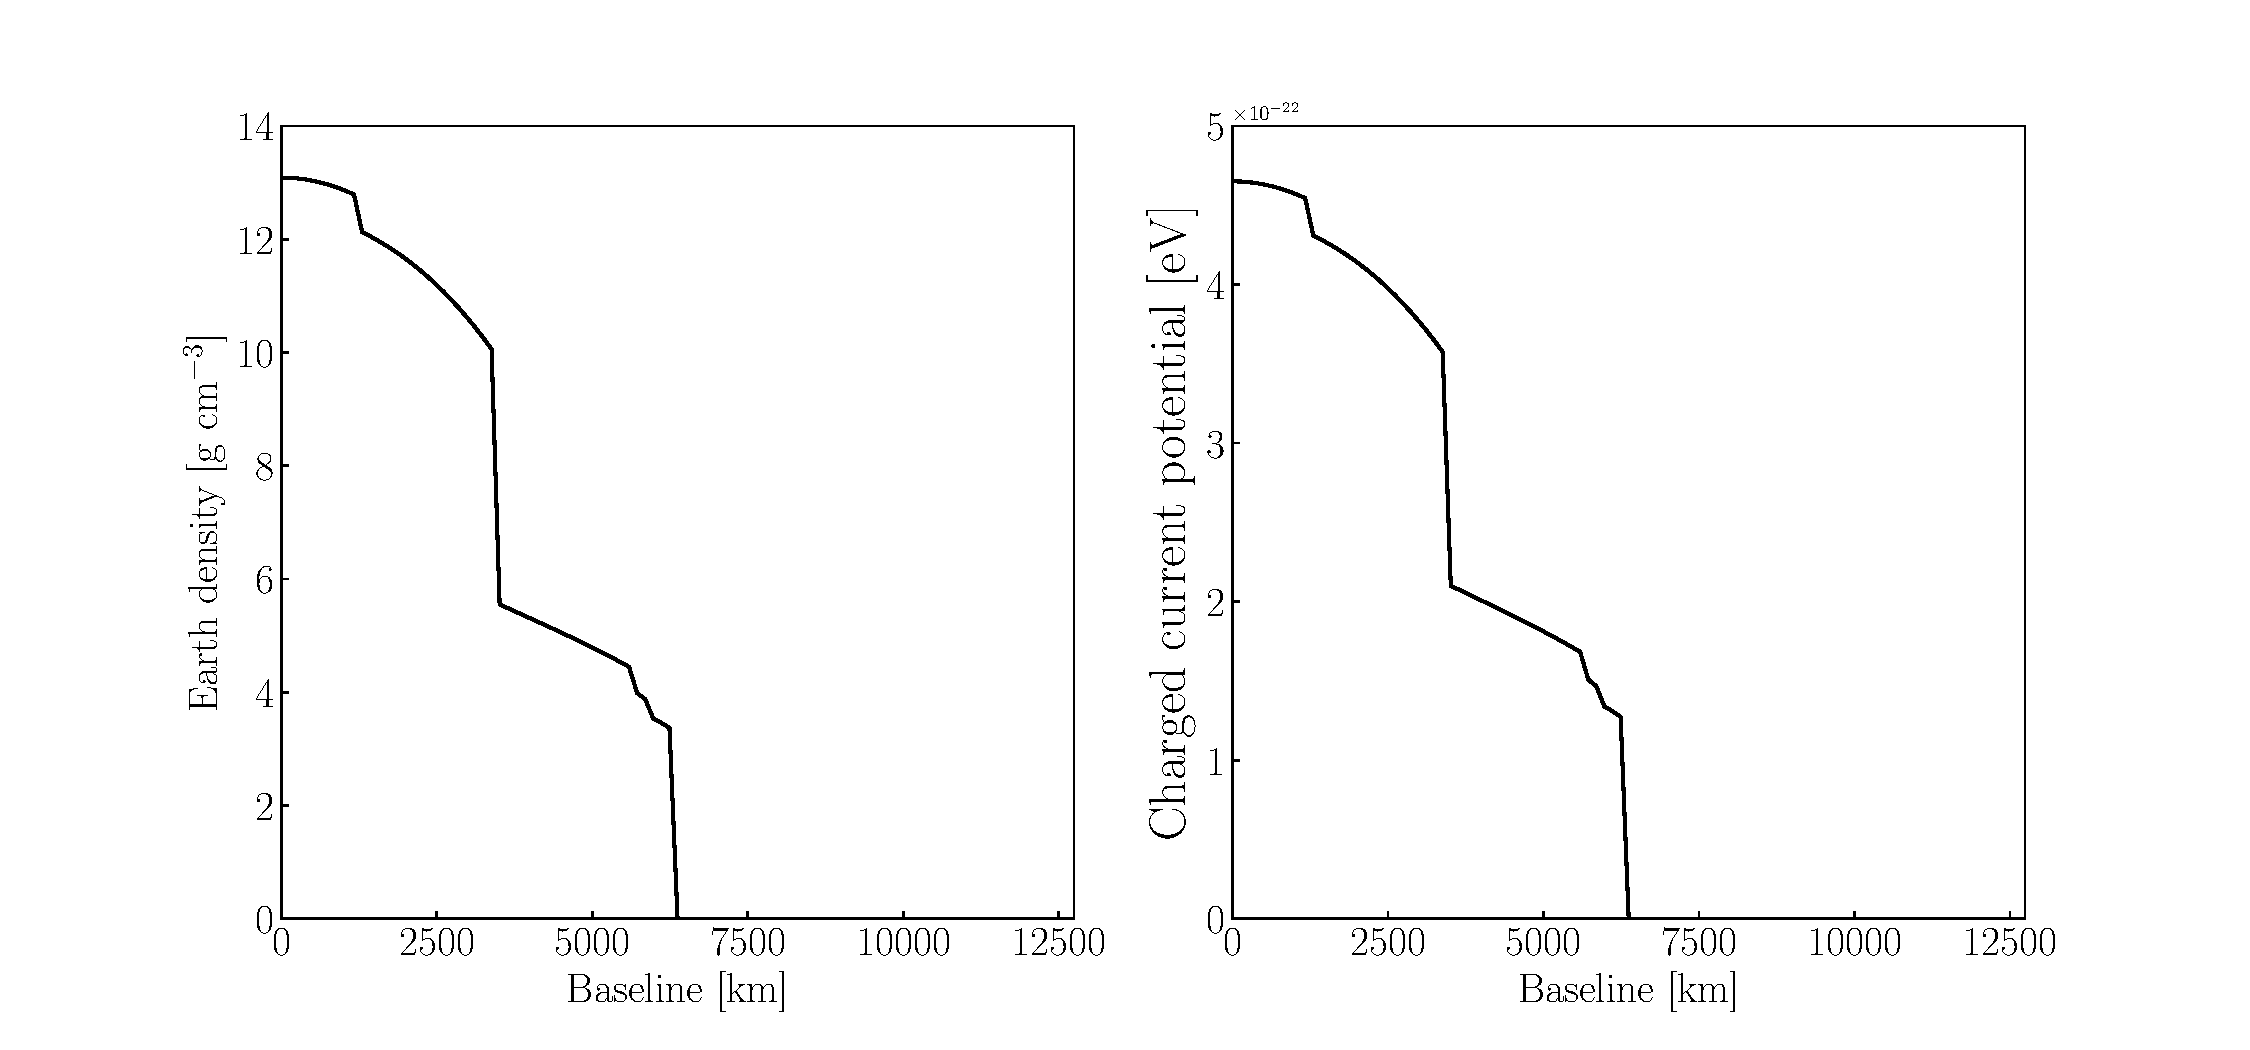
\includegraphics[width=0.7\textwidth]{figures/potential.pdf}
    \caption{\emph{Left panel:} Earth density asa function of distance from the core from the PREM~\cite{PREM}.
    \emph{Right panel:} $V_{CC}$ using the PREM density and 1/2 electrons per nucleon.}\label{fig:potential}
\end{figure}

Now, solving the Schrödinger equation with the Hamiltonian from Eq.~\ref{eq:H_3gen} with the matter potential from the PREM,
we obtain the nine combinations of probabilities through the Earth diameter. We note that due to our assumption of CP-invariance
(and thus, T-invariance), the probabilities $P_{\a\b}$ and $P_{\b\a}$ are identically equivalent. The result for \si{\GeV} neutrinos 
is shown in Fig.~\ref{fig:oscillations}.

\begin{figure}
    \centering
    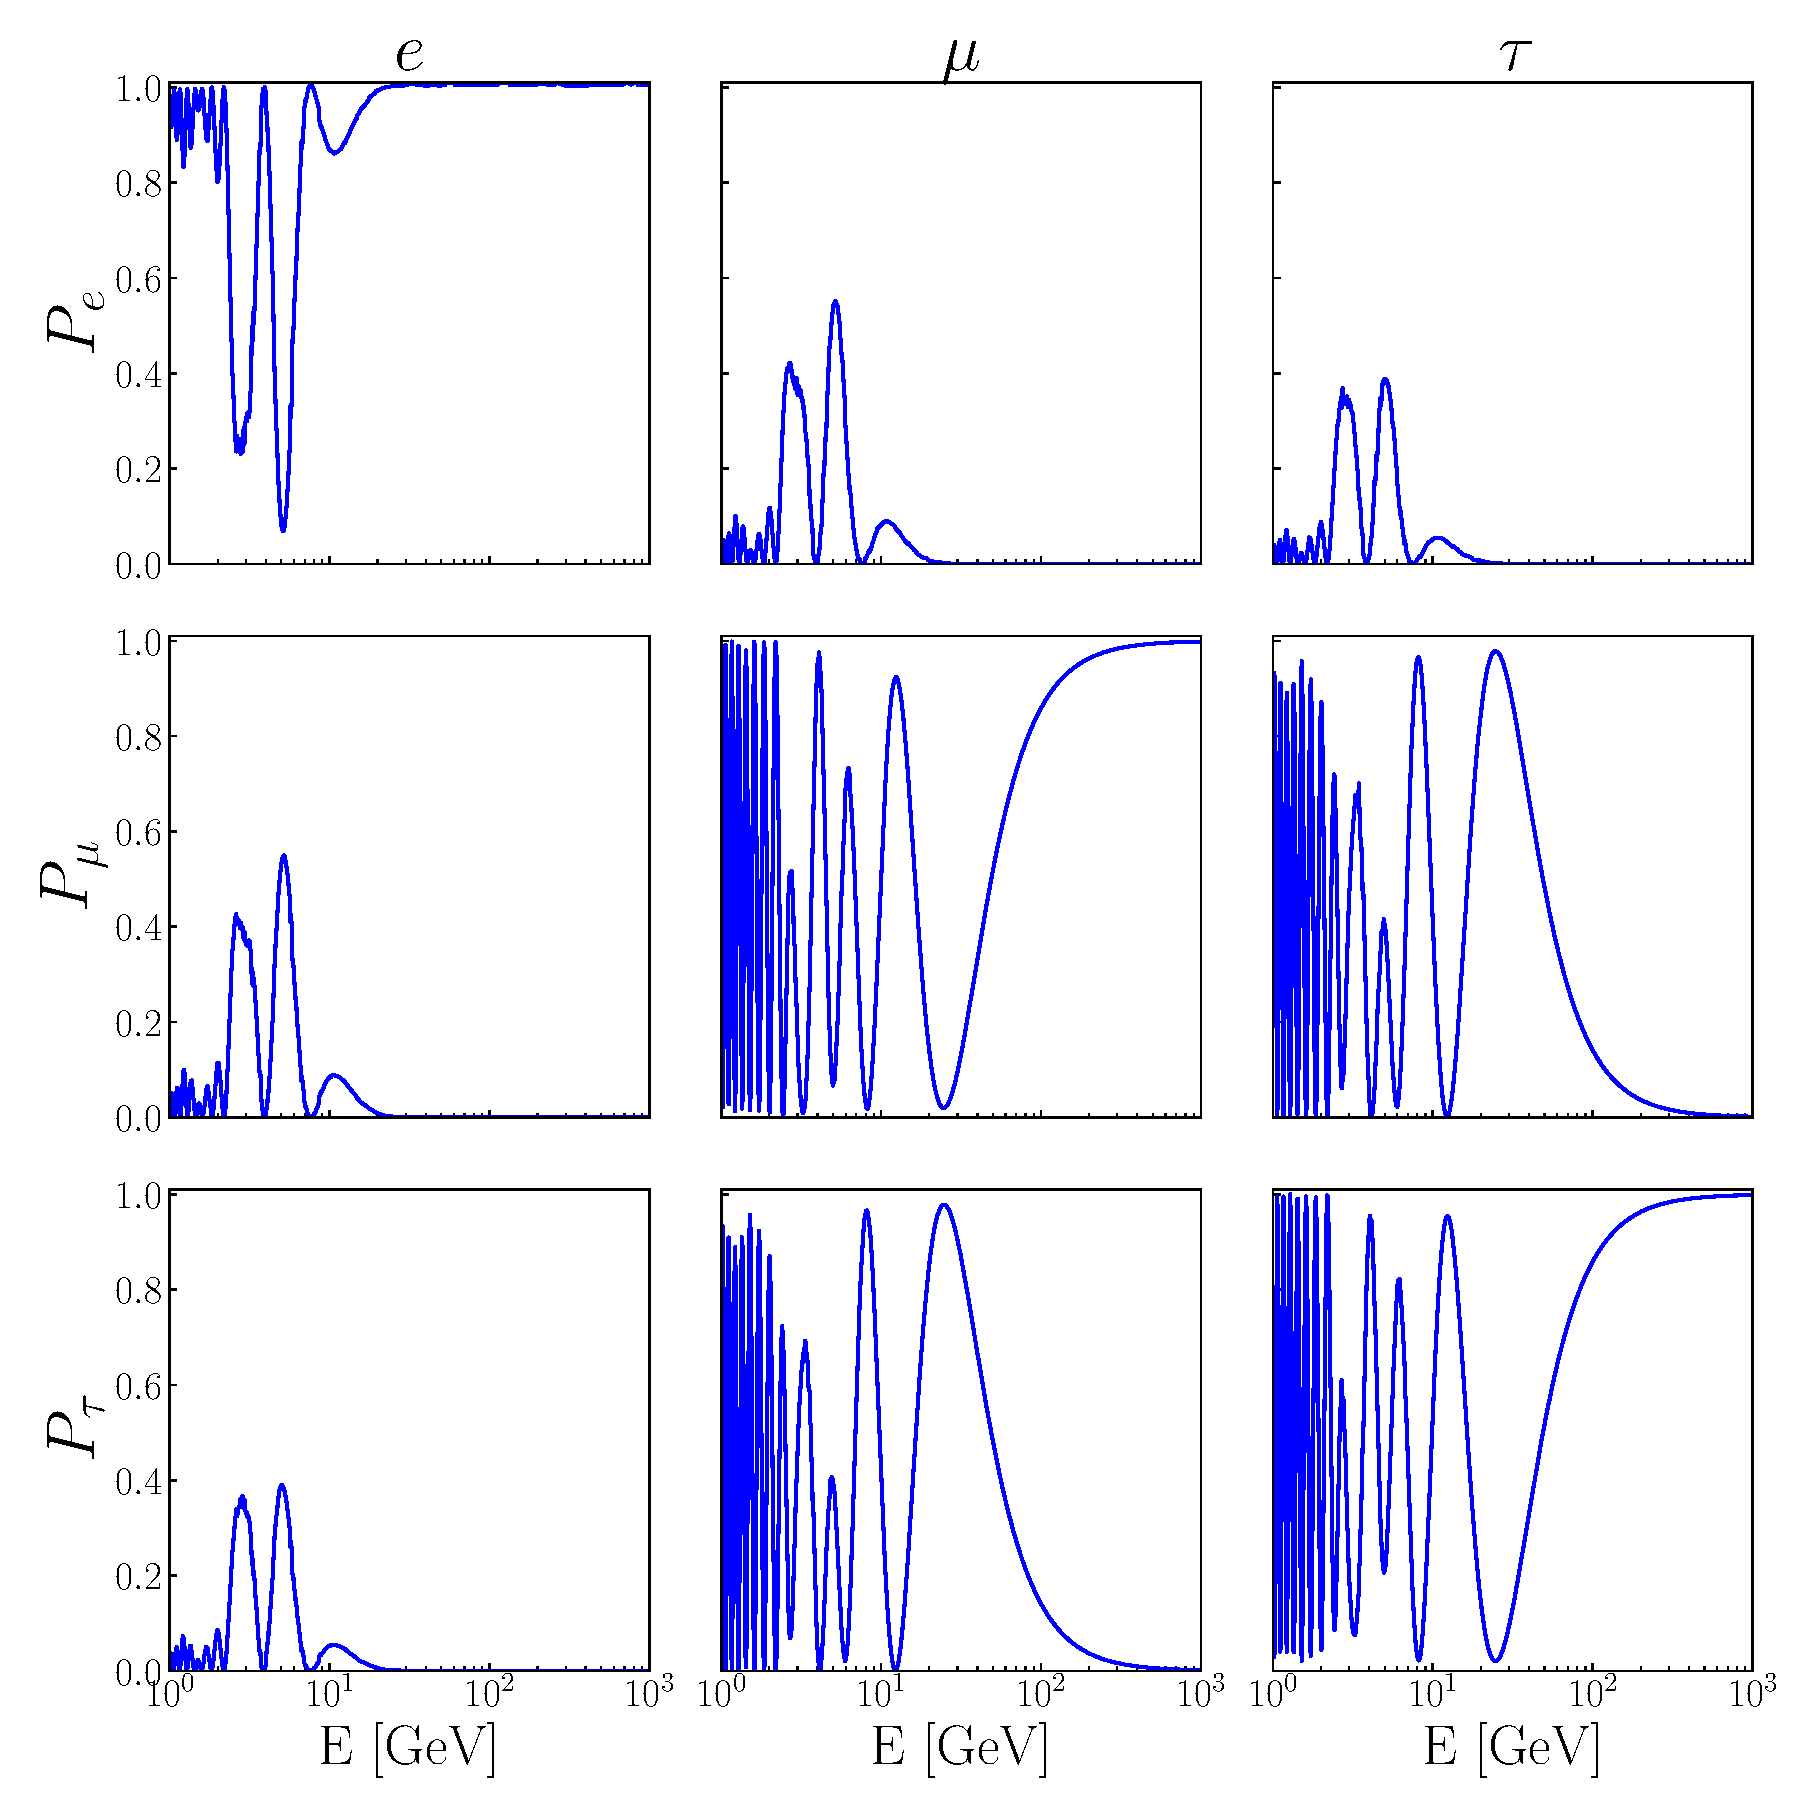
\includegraphics[width=0.7\textwidth]{figures/oscillations.pdf}
    \caption{}\label{fig:oscillations}
\end{figure}

Now we need to incorporate the \emph{zenith angle}, defined as the angle between the neutrino direction of travel and south.
This way, neutrinos traveling through the entire diameter of the Earth up through the South Pole are defined as `up-going', while
neutrinos that start at the South Pole are `down-going'. We will mostly work with the quantity $\cos{(\theta_z)}$.
Since we are interested in the matter effects, we reserve our IceCube study to up-going neutrinos, i.e. neutrinos with
zenith angle $-1<= \cos{(\theta_z)}<=0$. We now supplement our probability grid from Fig.~\ref{fig:oscillations} with the zenith dimension,
allowing us to fully see the Earth matter effect on the oscillations in full. This is shown in Fig.~\ref{fig:oscillograms}.

\begin{figure}
    \centering
    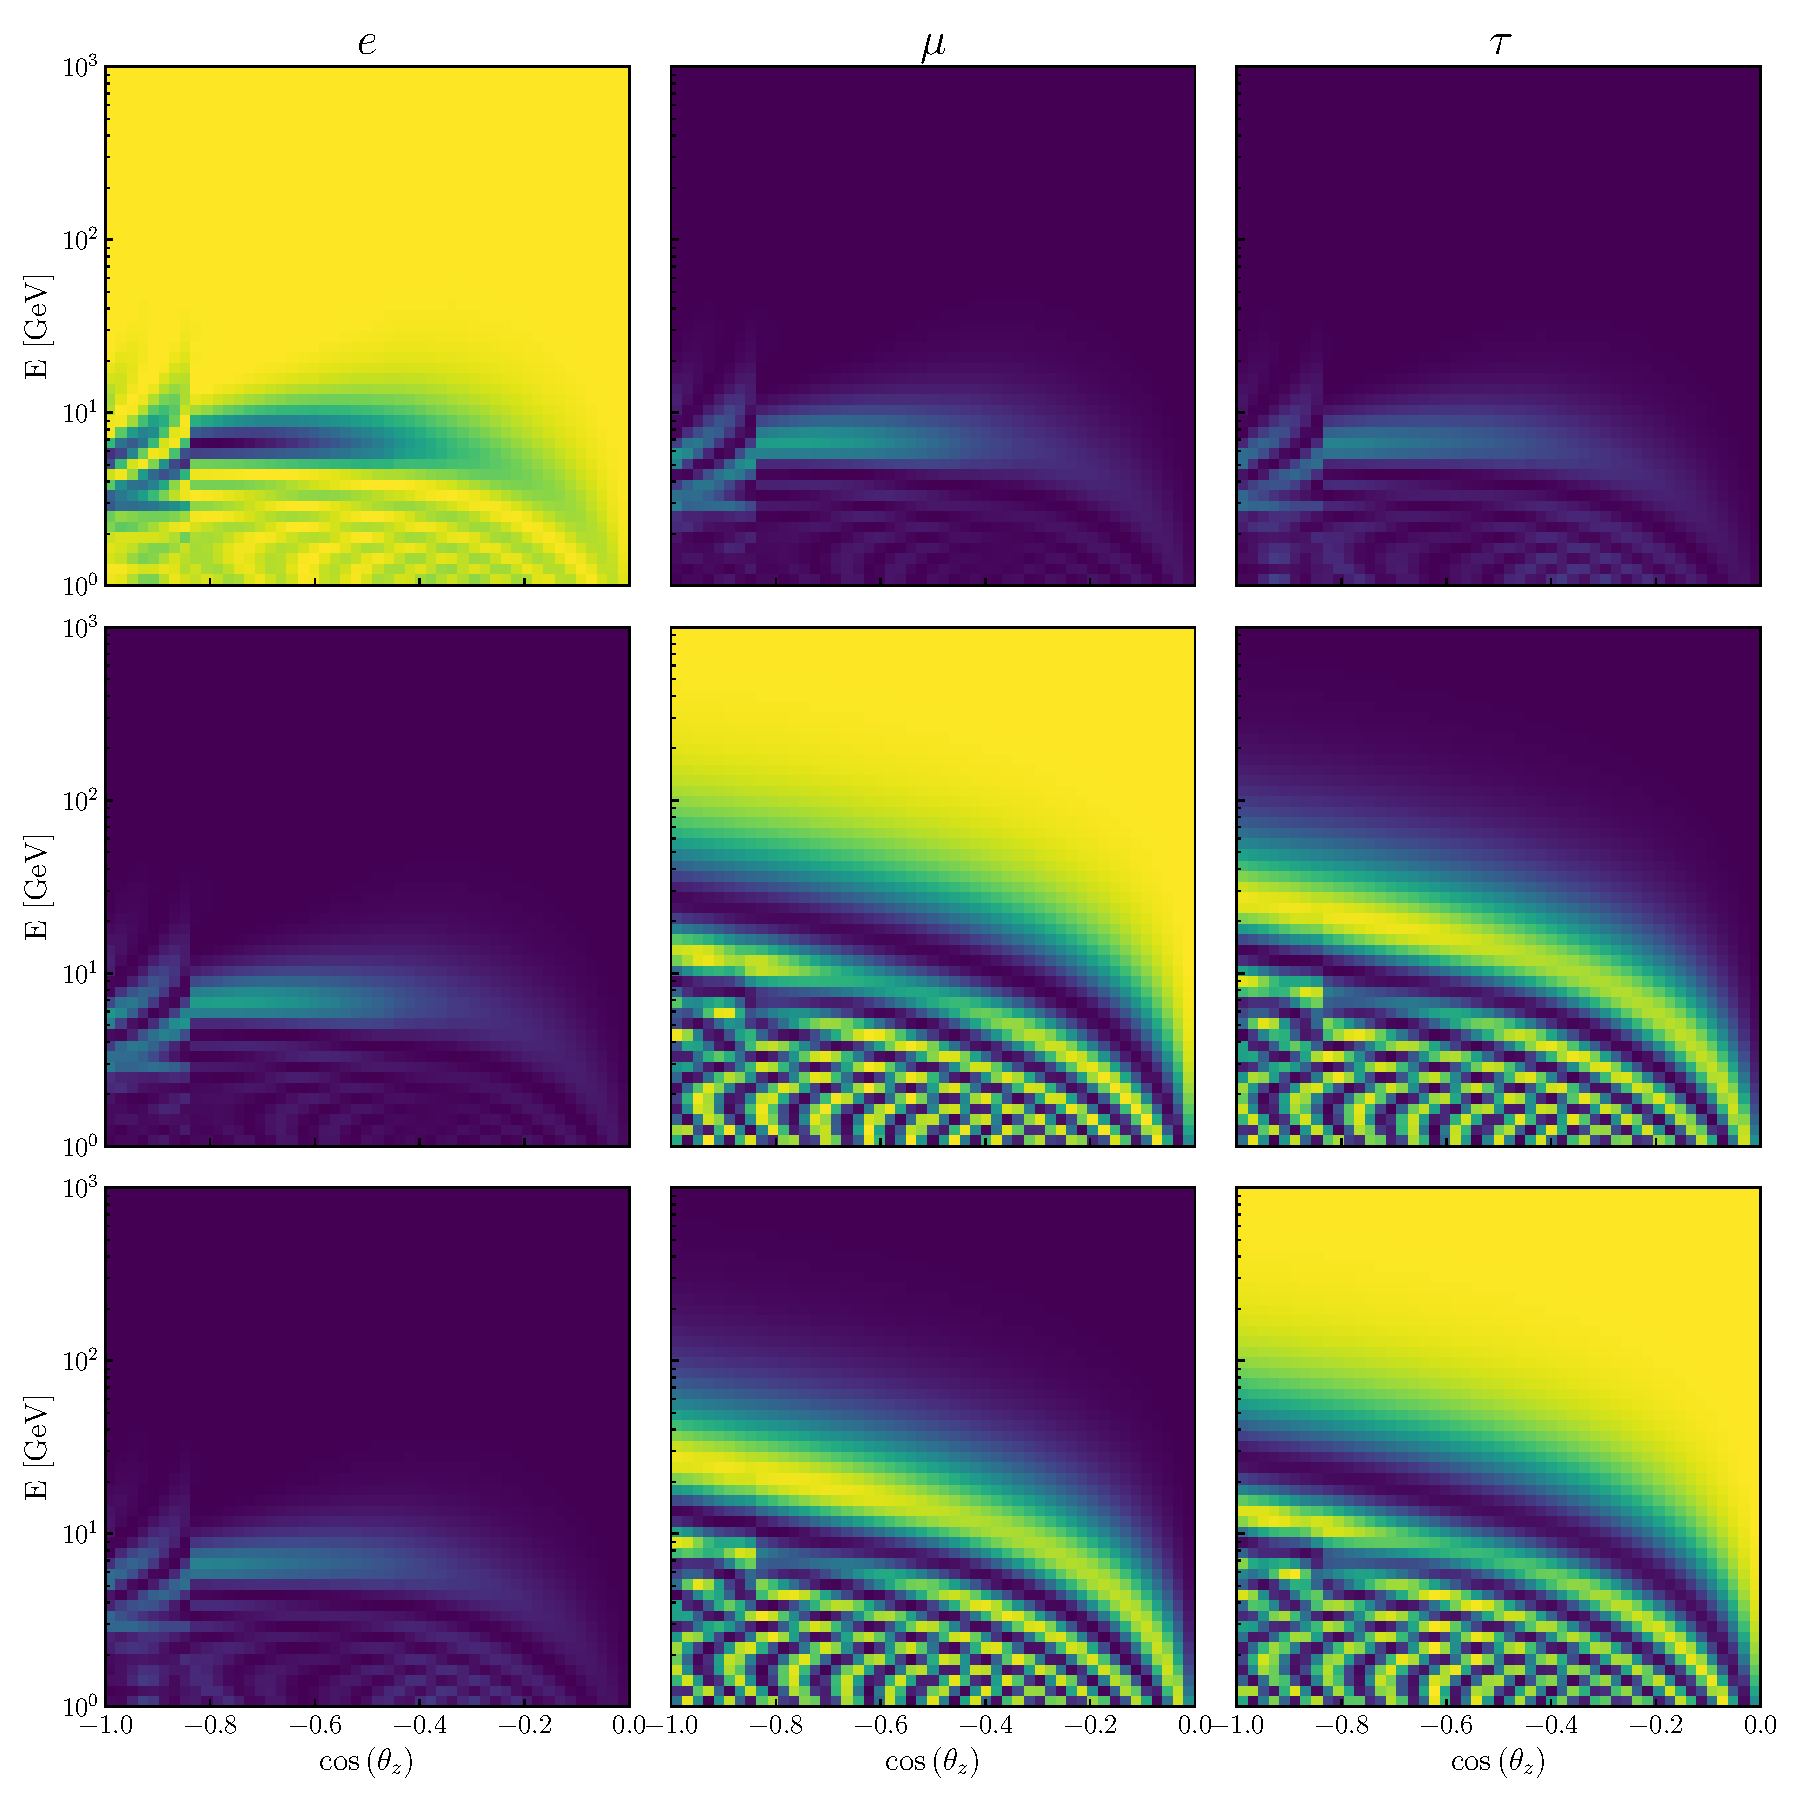
\includegraphics[width=0.7\textwidth]{figures/oscillograms.pdf}
    \caption{Oscillograms showing neutrino oscillations for all flavors in E-$\cos(\theta_z)$ space.}\label{fig:oscillograms}%TODO: redo finer
\end{figure}%TODO: remake with finer
The core-mantle boundary from Fig.\ref{fig:potential} is clearly displayed at $\cos{(\theta_z)} = -0.83$ as a sharp discontinuity for all flavors. 

% \end{document}